\chapter{Distributed Data Aggregation}
\section{Definition}
Data aggregation is a technique that consists, on its basis, in reduce the amount of data collected, reducing the resources needed to process it.  According to \cite{journals/corr/abs-1110-0725}, data aggregation is  considered a subset of information fusion, that aims at reducing the handled data volume. A more precise definition is given in the same report:
\begin{definition} An aggregation function $f$ takes a multiset of elements from a domain $I$ and produces an output of a domain $O$.
\begin{equation*} f : \mathbb{N}^I \to O \end{equation*}
\end{definition}
The order in which the elements are aggregated is irrelevant and a given value may occur several times. As the main goal of data aggregation, the aggregation function aims to summarize information. The result of an aggregation takes less space than the inputed multiset (element from $\mathbb{N}^I$).\\
Distributed data Aggregation or \textit{in-network} aggregation means that it is a task which is distributed among several nodes in the network. In contrary of a \textit{centralized} arquitecture, where a central node compute all the data and performs the aggregation function, a \textit{de-centralized} aggregation distribute the data, hence the effort to compute the aggregation function is reduced.
\subsection {Decomposable functions}
\todo{Correct definition? Need to specify more why decomposable functions could be computed in a parallel or distributed way}
For some aggregation function, one node may need to perform a single computation operation involving all the elements of the multiset, requiring more resources than the ideal ones. So, in order the distributed the effort to compute the multiset, there are some aggregation function that are decomposable. Meaning that, the effort could be done in a distributed way. A definition for decomposable function is also given in \cite{journals/corr/abs-1110-0725}:
\begin{definition} An aggregation function $ f : \mathbb{N}^I \to O$ is said to be self decomposable if, for some (merge) operator $\diamond$ and all non empty multisets $X$ and $Y$:
\begin{equation*}f(X \uplus Y) = f(X) \diamond f(Y) \end{equation*}
\end{definition}
The $\uplus$ denotates the standard multiset sum. The operator $\diamond$ is commutative and associative \cite{journals/corr/abs-1110-0725}. Some functions that are self-decomposable:
\begin{align*}SUM ({x}) &= x,\\
SUM(X \uplus Y) &= SUM(X)+SUM(Y).\end{align*}
\begin{align*}COUNT ({x}) &= x,  \\
COUNT(X \uplus Y)& = COUNT(X)+COUNT(Y).\end{align*}
\begin{align*}MIN ({x}) &= x,\\
MIN(X \uplus Y) &= MIN(X) \sqcap SUM(Y).\end{align*}
\begin{definition}
An aggregation function $ f : \mathbb{N}^I \to O$ is said said to be decomposable if for some function $g$ and a sel-decomposable aggregation function $h$, it can be expressed as:
\begin{equation*}f=g \circ h\end{equation*}
\end{definition}
As the definition above, stated in \cite{journals/corr/abs-1110-0725}, self decomposable functions are a subset of the decomposable functions. One example of a decomposable functions $AVERAGE$:
\begin{align*} 
AVERAGE(X) &= g(h(X)),\\
h({x}) &= (x,1),\\
h(X \uplus Y) &= h(X) + h(Y),\\
g((s,c)) &= s/c. \end{align*}
Another example is the $RANGE$ which gives the difference between the maximum and minimum value.


\subsection {Duplicate sensitiveness and idempotence} 
For some functions, the presence of duplicate results does not affect the result. Examples of this aggregation functions are $MAX$ and $MIN$, where the result on only depend on its \textit{support} set(obtained by removing all duplicates)\cite{journals/corr/abs-1110-0725}. Others, like $SUM$ or $COUNT$, the duplicate numbers are relevant. This propriety is called duplicate sensitiveness, it is relevante in distributed aggregation. Using an idempotent binary operator on the elements of the multiset helps obtaining fault tolerance \cite{journals/corr/abs-1110-0725}.
\begin{definition}
An aggregation function $f$ is said to be duplicate insensitive if for all multiset $M, f(M) = f(S)$, where $S$ is the support set of $M$.
\end{definition}
A taxonomy table of aggregation is in \cite{journals/corr/abs-1110-0725} and it is presented below.
\begin{center}    
\begin{tabular}{|c||c|c|c|}
    \hline
                                         &   \multicolumn{2} {|  c  |}{ Decomposable}                                               &    Non-decomposable \\ \hline
                                         &    Self-Decomposable      &                               &  \\ \hline
      Duplicate insensitive  &    $MIN,MAX$                  &     $RANGE$         &  $DISTINCT,COUNT$ \\ \hline
      Duplicate sensitive     &    $SUM,COUNT$           &     $AVERAGE$     &  $MEDIAN,MODE$ \\ \hline
    
    \end{tabular}
\label{Taxonomy of aggregation functions}
\end{center}

\section{Distributed Data Aggregation Algorithms}
\todo{Review DDA, Write the algorithms or just the type?}
In \cite{journals/corr/abs-1110-0725} is also presented a simple taxonomy of the existing algorithms that performe distributed data aggregation. First it is analyzed the algorithms from the communication prespective, i. e., the routing protocols and the intrisic topologies, afterwards, it is analyzed the computation issues, how the aggregation functions are computed by the algortihms.


\subsection{Communication}

\subsubsection{Hierarchy-based approaches} 
Traditionally, existing aggregation algorithms operate on a hierarchy-based communication scheme. This is \textit{structed} communication scheme. It is required to know in advance the topology of the network. A hierarchy communication tree is constructed, with several levels of nodes. In the root of the tree is a main repository of all data, denominated as sink. Besides the sink, other special nodes can be defined to compute intermediate aggregates, working as aggregation points that forwards their results to upper level nodes. There are generally two main phases, \textit{request} phase, corresponding to an aggregation request spreading through all the nodes, an the \textit{response} phase where all the nodes respond to the request sending their aggregation results. Some specific examples of these kind of communication are presented.\\
\\
\textbf{\textit{TAG}} The tiny AGregation algorithm that suits for ad-hoc networks described in \cite{madden2002tag}. This algrotihm requires the previous creation of a tree-based routing topology, and the continous maintenance of such routing structure in order to operate over mobile networks. TAG provides a SQL-like declarative language to the users. The algortihms consists of two main phases, the \textit{distribution} phase, i which a aggregation query is disseminated through all the spanning tree, and a \textit{collection} phase, where the values are aggregated. A waiting time is required to conclude this two phases.\\
\\ 
\textbf{\textit{DAG}} An aggregation scheme fro WSN is proposed in \cite{motegi2006dag} that aims to reduce the number of message losses. \todo{resume this shitty algorithm}\\
\\
\textbf{\textit{Sketches}} Algorithm proposed in \cite{considine2004approximate} that uses smal sketches. Based on the probabilistic counting sketches technique that estimates the number of distinct elements in a data collection. Like other algortihms of this type, is uses two phases: the sink propagates the aggregation request accross the network and then the results are collected back to the sick. In the first phase, all nodes compute theirs distances to the root, in the sencod phase the partial aggregates are computed across the routing structure, using the adapted counting sketch scheme, and send to the upper levels in sucessive rounds.\\
\\
\textbf{\textit{I-LEAG}} Cluster-based aggregation approach designated as I-LEAG is in \cite{birk2006veracity}. The routing structure of this algortihm is composed by a hierarchy of clusters or partitions. A single pivot is desginated for each cluster and the root is the pivot of the upper level cluster. This structure can be consider similar as we can see in networks with \textit{super-peers}, but organized in a tree structure. The algorithm works as follows: each cluster check local conflicts that are reported to the pivot, then the pivot computes the new aggregate and multicast the result, each node must forward the received result to the nodes outside the cluster.\\
\\
\textbf{\textit{Tributary-Delta}} 
This approach mixes the tradional use of tree and multi-path routing schemes, dividing the network in two routing regions: \textit{delta}(multipah) and \textit{tributary}(tree). Use tributaries in regions with low rate of message losses to take advantage of tradiontal tree schemes and delta in regions with higher rate of message losses(mostly regions near the sink with the aggregate of several nodes).
\todo{resume other approachs}
\todo{Ring Based Approachs, Flooding and Randomized necessary or relevant?, IDEA: state the hierarchy and gossip approach and then the hybrid aproach combining the two}

\subsubsection{Gossip-based approaches}
This type of approach is reffered as an \textit{unstructed} approach, contrary of a aforementioned \textit{structed} approachs. In this type of scheme there is no previous knowledge of the topology of the network or any specific structure. The information or messages are commonly disseminated accross the network without follwing any specifc topology, the informartion it is passed node to node, or nodes, like a infectious disease or a gossip,i.e., a "infected" node sends a message to a random subset of nodes. This type scheme tend to allow a robust(fault tolerant) and scalable information dissemenation over all the network\cite{journals/corr/abs-1110-0725}\\
\\
\textbf{\textit{Push-Sum Protocol}}  Push-sum protocoI\cite{kempe2003gossip} is a gossip-based protocol to compute aggregation functions. Along discrete times $t$, each node $i$ maintains and propagates information of a pair of values $(s_ti,w_ti)$ where $s$ represents the sum of the exchanged values and $w$ the weight associated. In each iteration, a neighbor is choosen uniformly at random and half of the actual values are sent to the target node and the other hald to the node itself. Upon reveived, the local values are updated, adding each value from a received pair to its local component\cite{journals/corr/abs-1110-0725}.\todo{review this definition, too much alike}

\subsubsection{Hybrid approaches} 
Hybrid approaches propose a solution that merge both hierarchic and gossip-based approachs, using the high accuracy and efficiency of the hierarchic based schemes and the robustness of the gossip approachs. In the disadvantages of one approach , the other one has it as an advantage, Hybrid approachs aim to merge the advantages of both schemes to elimanate both disadvantages.\\
\\
\textbf{\textit{Chitnis et al, 2008}} Chitnis et al.\cite{chitnis2008aggregation} proposed an hybrid approach, using TAG as an hierarchy-based approach and Push-Sum as a gossip-based protocol. This hybrid approach divides the network node in groups. Inside each group, a gossip-based protocol is used. In each group, a leader is elected to further performe a hierachic communication with other  leaders nodes regarding the aggregation results from the gossip group. 

\subsection{Computation}
\subsubsection{Hierarchical}
The input is separted into groups so it can be computed in a distributed hirarchical way.  Depends on the previous formation of a communication structure such as tree or cluster. Some node work as \textit{forwarders}, just forward data to upper levels of the hierarchy, and others work as \textit{aggregators}, apply the aggregation function directly to all received input and then work as a normal \textit{forward} node. This class of algorithms allow any decomposable function with high accuracy without the presence of faults. Algortithms of this class were aforementioned.
\subsubsection{Averaging}
This class of computation scheme is based on a iterative computation of partial aggregates, where all nodes share their results among the network and all of them contribute for the final result. This scheme provides high accuracy, considering that all nodes converge to the same result. One example of algorithms of this class, are the ones with gossip base communication scheme, since the results of the aggregates could be share randomnly with the neighbor nodes. Due to its nature, Averaging algorithms tend to by highly robust, i.e., tolerant to faults on opposite of the structed algrotihms. Decomposable and duplciate sensitece functions can be be computed in this class.\\
\todo{specify the mass conservation concept?}\\
\textbf{\textit{Push-Pull Gossiping}} Similar to the aforementioned \textit{push-sum protocol}, the push-pull gossiping\cite{jelasity2004epidemic} performes an averaging process. This algortihm executes an epidemic protocol to perform a pari-wise exchange of aggregated values between neighbor nodes\cite{journals/corr/abs-1110-0725}. In periodic intervals of time, a node send its value to a randomly selected node and waits to receive a result back, the response from the selected node. Afterwards, an average with the new value and the present value its perfomed in order to calculate and store a new one. When a node receives a value from another node, the same process is performed, send the current value and calculate a new one from the average of the received value and the current one.\\ 
\\
\textbf{\textit{DRG(Distributed Random Grouping)}} This approach \cite{chen2006robust} randomly creates groups across the network in which aggregates are sucessfully computed. There are three modes a node can performe:\textit{leader,idle} and \textit{member} which corresponds to three phases. First every node is in \textit{idle} mode, them every node broadcasts a Group Call Message, pretending to be a group leader(with a pre-defined probability associated ) and waits for members. The nodes who receives the group call, respondes to the first one received with a JACK(Joining Acknowledgment) tagged with their aggregated value becoming a member of the group. Finally, the \textit{leader} gather all the aggregated values, computing the aggregation function($AVERAGE$) and broadcasts a Group Assignment Message with the  final result. Every group member waits unit it receives the result from the leader to update its local value and them returns to  \textit{idle} mode.\\
\\
\textbf{\textit{Flow Updating}}\todo{finish this shitty algorithm}\\

\subsubsection{Sketches}
Algrorithms based on the use of an auxilary data structure with a fixed size that holds a \textit{sketch} of all network values. Input values are used to create \textit{sketches} that aggregated across the network, using specific operations to update and merge them. The agregation could be done using multiple paths. This type of algorithms enable operations of order and duplicate insentitive. The computational cost of this class depends mainly on the resources used to produce the result by the estimator and the complexity of the operations to produce the \textit{sketches}. This kind of algorirthms tend to be very fast, depending on the dissemination protocol used to propagate the sketches, but lack accuracy because they are based on probabilistic methods.\\
\\
\textbf{\textit{RIA-LC/DC}} Algorithm proposed in \cite{fan2008efficient}, a multi-path routing aggregation approach. The algrotihm consists of two phases. First a aggregation request is sent by the sink throughour the whole network, creating a multipath routinh hierarchy. Second, starting in the lower leves, each node generates a \textit{sketch} correspondent to its current state and sent it to the nodes in the upper level. The node that receives the \textit{sketch}, creates a new one combining tis current value and the received \textit{sketch} and send it to the upper node until the top is reached where the sink computes the aggregation estimate.
\\
\textbf{\textit{Extrema propagation}}
This approach redices the computation of an aggregation function\cite{journals/corr/abs-1110-0725}. A vector $x_i$ of $k$ random number is created at each network node $i$. Random numbers are generated according to a known random distribution, using the node initial value as an input parameter. The execution of the algorithm consists os the computation of the pointwise minimum between all exchagend vectors. At each node, the obtaind vector is used as a sample to produce an aproximation of the aggregation result. This algorithm is focused ob obtaining a fast estimate, tather than an accurate one. 
\subsubsection{Digests}
This class of algrotihms allow the computation of more complex functions like meadian or mode than the normal aggregation function such as $SUM$ or $AVERAGE$. This algrotihms produces a \textit{digest}, data structure with a bounded size that holds an aproximation of the statistical dristribution of input values in the whole network, that summarizes the system data distribution, an histogram. The accuracy of this calss of algortihms depends mostly on the quality and size of the obtained \textit{digest}. Usually requires more resources.\\
\\
\textbf{\textit{Q-Digest}} This aggregation scheme allows the approximation of complex aggregation function in WSN is proposed in \cite{shrivastava2004medians}. Uses an hierarchical routing topology to build and disseminate quantile digests. Each node maintains a quantile digest of the data avilabe, which are built in a botton-up fashion by merging received digest from lower nodes(children nodes). This new quantile digests are compressed according to a specific compression factor. Aggregation functions are computed by manipulating and traversing the quantile structure acording to a specific criteria.\\
\\
\textbf{\textit{Equi-Depth}} Gossip-based approach described in  \cite{horowitz2003estimating}. The scheme executes a  gossip protocol and merge specific function on the exchanged data. Each node keeps a list of $k$ value or \textit{digests}, initially set to its input value. Each node randomly chooses a neighbor to exchange the digest to merge with its own. This round is executed several number of times, producing an aproximation of the network distribution of values. There are four merging techniques \textit{swap, concise, equi-with histograms} and \textit{equi-depth histograms} that are detailed in \cite{journals/corr/abs-1110-0725}.
\textbf{\textit{Adam2}}
Adam2 is a gossip based algorithm to estimate the statistical distribution of values across a decentralized system\cite{sacha2010adam2}. Each node can decide to start an instance of Adam2 where each instance is uniquely identified by its starting node. The statrting node $i$ initializes the interpolation set $H_i$(composed of $k$ pairs of values $(x_k,f_k)$ where $x_k$ represents an interpolation point and $f_k$ the fraction of nodes with value less or equal to $x_k$). The interpolation is initialized by seting $f_k$ to 1 if the node attribute reading $v_i$ is less or equal than the corresponding interpolation value $x_k$, 0 otherwise. Node store a set of interpolaton points for each running algorithm instance.  A new node that learning about the new instance performes a initializtaion ant then starts participating in the protocol. The sets are exchanged like push-pull, the sets are merged by averaging the fraction at each interpolaiton poin. After a predefined number round the CDF is approximated by interpolating the point of the resulting set.



\section{WSN Data Aggregation}
Distributed Data Aggregation in WSN is an widely study subject, with several works and proposed solutions. Distributed aggregation adquires a special importance in WSN, since the sensor are low resources devices so the effort distribution is quite mandatory. The aggregation techniques reduce the amount of data communicated within a WSN and thus conserve battery power \cite{castelluccia2005efficient}.Periodically, as measurements are recorded by individual sensors, they are been collected and processed to produce data representative of the entire WSN.  An natural approach is consider that the sensor send the measured data to special sensor nodes, i.e., aggregator nodes \cite{castelluccia2005efficient}. In \textit{in-network} aggregation nodes forward the aggregated data to a sink that store it.\\
\begin{figure}[h]
\centering
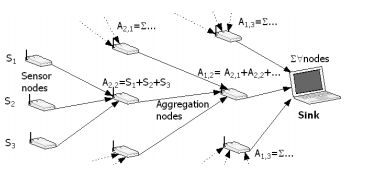
\includegraphics[width=0.5\textwidth]{/Users/rafaelremondes/UM/MEI/Thesis/DistributedAggregationAlgortihmsSM/Writing/Images/INA}
\caption{\label{fig:INAaggregation} Principle of in-network aggregation}
\end{figure}
An example of \text{in-network} aggregation in WSN is in  \cite{castelluccia2005efficient}. In this model, it is assumed that all nodes ate potential aggregators and that data gets aggregated as they propagate towards the sink. The aggregation is set as must being simple not involve any expensive or complex computation. The aggregation requires all sensors to send their data to the sink within the same sampling period so there is a need for a global so that all node can synchronize. Another study is in \cite{Girao2004c}, where a special kind of distributed aggregation is proposed, \textit{Concealed Data Aggregation}. This type of aggregation is defined as an approach than promises the combination os end-to-end security and \textit{in-network} aggregation. In \cite{chan2006secure} it is assumed a general multi-hop network with a set $S={s_1....s_n}$ of $n$ sensor nodes anda a single base station $R$. The aggregation is performed over an \textit{aggregation tree} which is the directed tree formed by the union of all the paths from the sensors nodes to the base station. Another WSN distributed aggregation scenario is presented in \cite{yu2009distributed}. The network model consist of a $n$ sensor nodes and one base station that is also called a sink. Each sensor node can send or receive data to or from all directions. It is assumed that all nodes have the same transmission range for simplicity. A node can either receive or send data at a time and it can receive a data packet correctly when it hears only this packet at that moment.


\section{Smart Metering Aggregation Model} 
There are two main architectures for smart metering considering data aggregation  are \textit{centralized} and \textit{distributed} or \textit{ decentralized}\cite{journals/spm/ErkinTLP13}. In \textit{centralized} fashion, the meters just sense the data, afterwards, it is sent to a central aggregator with higher computation power that holds a central database. In a \textit{decentralized} way, the aggregation role is distributed among several meters, not all of then. This type of aggregation is also called  \textit{in-network} aggregation \cite{Girao2004c}\cite{Castelluccia05efficientaggregation}. The aggregation node in this scheme communicate the calculated energy consumed to an appropriate party such as a energy producer. Typically, this communication occurs once per billable period \cite{journals/spm/ErkinTLP13}. As introduced before, the architecture chosen for this work is \textit{de-centralized} due to the nature of the aggregation algorithms.\\
In the literature, it is possible to find some particular studies. Keita Suzuki \textit{et al} \cite{DBLP:conf/isgteurope/SuzukiNYKMKA13}  presents a particular case in a office building in Japan(Heating ventilation and air conditioning facilitie,HVAC) where existis the need to aggregate power curtailments from hundred or thousands of distributed HVAC facilities. Several smart meters where placed, connected to a Gateway that receives the consumption data for daily or monthly billing.  The Gateways are connected to a central ADR, Aggregation Cloud, which aggregates all the consumption.\\
Another work using a \textit{de-centralized} way is in Rottondi \textit{et al}\cite{rottondi2012}.  The smart meters generate the energy consumption measurements, the Gateways securely aggregate the metering data and external parties access the aggregation results. Each meter is directly connected to a Gateway, receiving data from a limited number of meters. At regular time intervals, 15 min in this case, the meter generate a measurement and send it to the Gateway. The overall scheme is presented in \ref{fig:meterArchitecture}.
\begin{figure}[h]
\centering
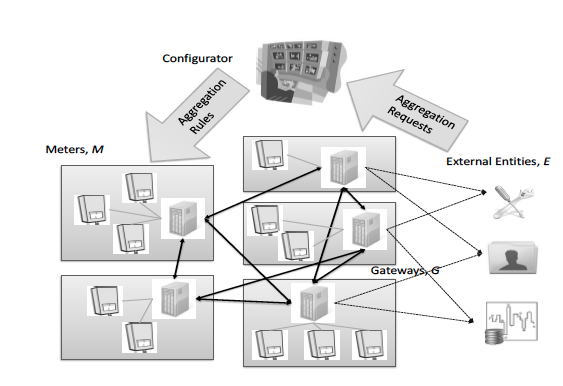
\includegraphics[width=0.5\textwidth]{/Users/rafaelremondes/UM/MEI/Thesis/DistributedAggregationAlgortihmsSM/Writing/Images/meterExample}
\caption{\label{fig:meterArchitecture} The functional nodes of the architecture}
\end{figure}

